\subsection{Part A}
\[ r - 30 = 2.0(t - 5) \]
\[ r - 30 = 2.0(5.4 - 5), \enspace r = 30.8 ft \]
\begin{center}
	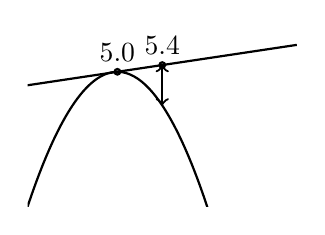
\begin{tikzpicture}
		\begin{axis}[thick,smooth,no markers, hide axis, xmin=-0.5, xmax=1.0, ymin=0.0, ymax=0.5, height=5cm, width=5cm]
			\addplot[samples=100, domain=-1.0:1.0] {-\x*\x + 0.25};
			\addplot[samples=100, domain=-1.0:1.0] {0.05*\x + 0.25};
			\draw[arrows=<->] (0.25, 0.2625) -- (0.25, 0.1875);
			\draw (axis cs:0.0, 0.25) circle(1pt) node[above] {$5.0$};
			\draw (axis cs:0.25, 0.2625) circle(1pt) node[above] {$5.4$};
		\end{axis} 
	\end{tikzpicture}
\end{center}
The approximation is above the actual value, because the line approximation will overshoot the decreasing (concave down) function.

\subsection{Part B}
\[ r(5) = 30, \enspace r'(5) = 2.0 \]
\[ \frac{dV}{dt} = \frac{d}{dt} \frac{4}{3}\pi r^3 = 4 \pi r^2 r' \]
\[ 4 \pi (30.0)^2(2.0) = 7200\pi \, ft^3/min \]

\subsection{Part C}
\[ \int_{0}^{12} r'(t)\,dt \approx \sum _{i=1}^{6}r'(t)_{i}\,\Delta t_{i} \approx \]
\[ (0.5)(1) + (0.6)(4) + (1.2)(2) + (2.0)(3) + (4.0)(2) = 19.3 \, ft\]
\underline{$\int_{0}^{12} r'(t)\,dt$} represents the number of feet the balloon has expanded (in radius) past it's original condition, and it is \textbf{not} the absolute radius of the balloon.

\subsection{Part D}
\begin{center}
	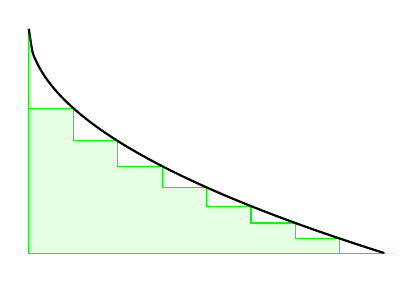
\begin{tikzpicture}
		\begin{axis}[
			height=5cm,
			width=7cm,
			xmin=0, xmax=1, ymin=0,ymax=1,
			hide axis,
			enlargelimits=true,
			clip=false,
			domain=0:1,
			axis on top
			]
			\addplot [draw=green, fill=green!10, const plot mark right, samples=9, domain=0:1] {1 - sqrt(\x)}\closedcycle;
			\addplot[smooth, thick,domain=0:1,samples=100]{1 - sqrt(\x)};
		\end{axis}
	\end{tikzpicture}
\end{center}

The RHS will under approximate the graph because it's slope is always negative, meaning any nonzero area under the curve from the right will undershoot it travelling left.
